\chapter{Impl\'ementation de la solution}

\section{Introduction}

Ce chapitre aborde comme sujet les choix technologiques et les outils pour l'impl\'ementation de notre solution ainsi que les captures d'\'ecran des diff\'erents fen\^etre r\'ealiser et les tests de validation effectu\'es sur les modules d\'evelopp\'es.

\section{Environnement logiciel}
L'environnement logiciel utilis\'e pour la r\'ealisation de notre projet est pr\'esent\'e dans le tableau suivant :

\begin{table}[H]
\begin{center}
\begin{tabularx}{\textwidth}{ |l|X| }
\hline Outil & Description \\\hline \hline
JDK 1.8 & Java Development Kit (JDK) d\'esigne un ensemble de biblioth\`eques logicielles de base du langage de programmation Java.\\ \hline
Intellij IDEA & Environnement de d\'eveloppement int\'egr\'e (IDE).\\ \hline
Visual Studio Code & Environnement de d\'eveloppement c\^ote frontend.\\ \hline
Android Studio & Environnement de d\'eveloppement pour d\'evelopper des applications mobiles Android.\\ \hline
GitBash & C'est une ligne de commande dans laquelle on peut ex\'ecuter les commandes git.\\ \hline
Zeplin & C'est un outil de design des fonctionnalit\'es. Permet de collaborer entre les designers et les d\'eveloppeurs frontends, facile, efficace et permet de gagner du temps.\\ \hline
Postman & Est actuellement l'un des outils les plus populaires utilis\'es dans les tests d'\gls{API}.\\
\hline
\end{tabularx}
\caption{Environnement logiciel}
\end{center}
\end{table}

\section{Architecture technique du syst\`eme}

Notre syst\`eme se base en totalit\'e sur l'architecture orient\'e service et plus pr\'ecis\'ement sur l'architecture \gls{REST}. C'est un style d'architecture pour la conception d'applications faiblement coupl\'ees sur \gls{HTTP}, souvent utilis\'e dans le d\'eveloppement de services Web.

Une \'etude qui a faite par l'entit\'e \gls{DF}, ils sont convaincu d'adapter quelques technologies \& outils dans tous leur projets. 

La figure suivante repr\'esente les technologies \& les biblioth\`eques essentiels utilises dans notre projet (Prospektor).

\begin{figure}[H]
	\center{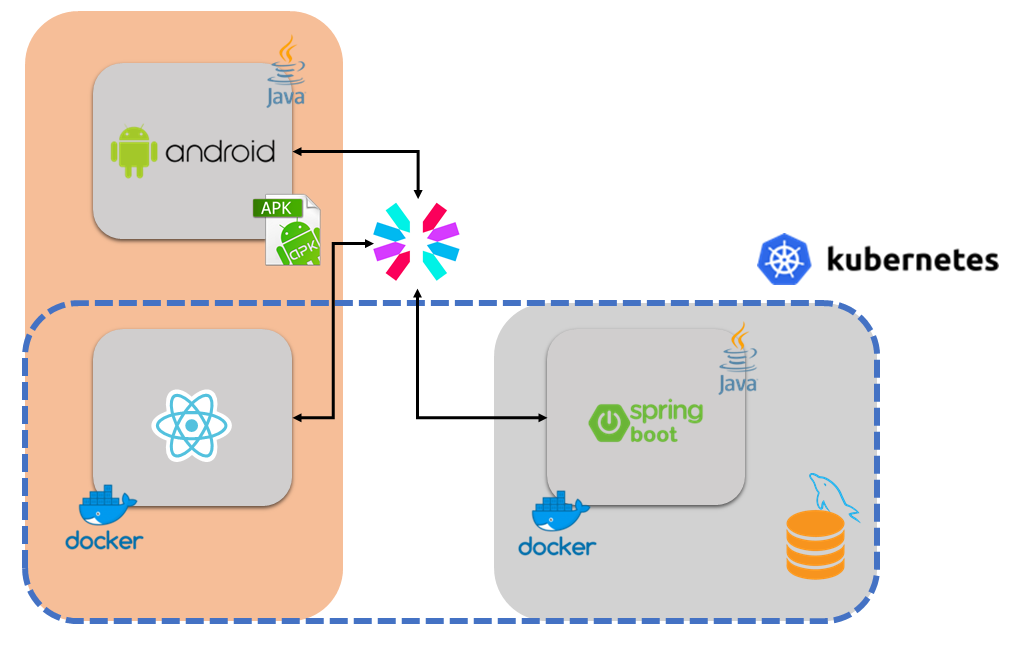
\includegraphics[width=\textwidth]{Figures/achitec-tech.PNG}}
	\caption{\label{fig:my-label} Architecture technique du syst\`eme}
\end{figure}

Maintenant, on va expliquer l'utilit\'e des technologies utilises dans notre impl\'ementation. 

\subsection{Couche BackEnd}

Pour la partie backend, on va utiliser les technologies suivantes :

\begin{itemize}

\item \textcolor{spring}{SpringBoot} : est un framework Java open source utilis\'e pour cr\'eer un Micro Service. Il est facile de cr\'eer des stand-alone applications. Spring Boot contient une prise en charge compl\`ete de l'infrastructure pour le d\'eveloppement d'un micro-service et vous permet de d\'evelopper des applications d'entreprise.

Pourquoi Spring Boot est un excellent choix pour Prospektor :

\begin{itemize}
\item Spring Boot est bas\'e sur le framework Spring.

\item Les modules centraux et centraux des \'ecosyst\`emes Spring sont stables pendant une longue p\'eriode et la plupart des modifications sont compatibles avec les versions ant\'erieures.

Bas\'e sur la machine virtuelle Java

\item Spring Boot et les principaux modules Spring de l'\'ecosyst\`eme sont des logiciels open source. Cependant, il est fortement entretenu et soutenu par Pivotal, une soci\'et\'e proposant des plates-formes et des outils permettant de cr\'eer de meilleurs logiciels.

\item Son utilisation est gratuite.

\item Ex\'ecutez-le sur votre propre serveur, machines virtuelles, conteneurs ou h\^ote sur Heroku, AWS ou similaire. C'est \`a toi de decider.

\item Avec Spring, vous pouvez facilement connecter votre application \`a des bases de donn\'ees relationnelles, \`a des bases de donn\'ees NoSQL ou \`a des services de file d'attente.

\item Prend en charge Oracle, PostgreSQL, MySQL, MongoDB, Redis, Solr, ElasticSearch, Rabbit MQ, ActiveMQ et bien d'autres encore.

\item Avec Spring Boot, vous pouvez d\'evelopper des applications Web rendues typiques c\^ot\'e serveur, RESTful et d'autres API Web, ou m\^eme cr\'eer des travaux par lots et des applications de ligne de commande standard.

\item Les d\'eveloppeurs adorent programmer avec Spring Boot. Ils sont plus productifs, b\'en\'eficient des avantages de l'\'ecosyst\`eme Spring et de la tranquillit\'e d'esprit des syst\`emes de production en fonctionnement.
\end{itemize}


\item \textbf{Swagger} : nous permet de d\'ecrire la structure de nos API afin que les machines puissent les lire. La capacit\'e des API \`a d\'ecrire leur propre structure facilite aux d\'eveloppeurs frontend la communication avec nos serveurs.

\begin{figure}[H]
	\center{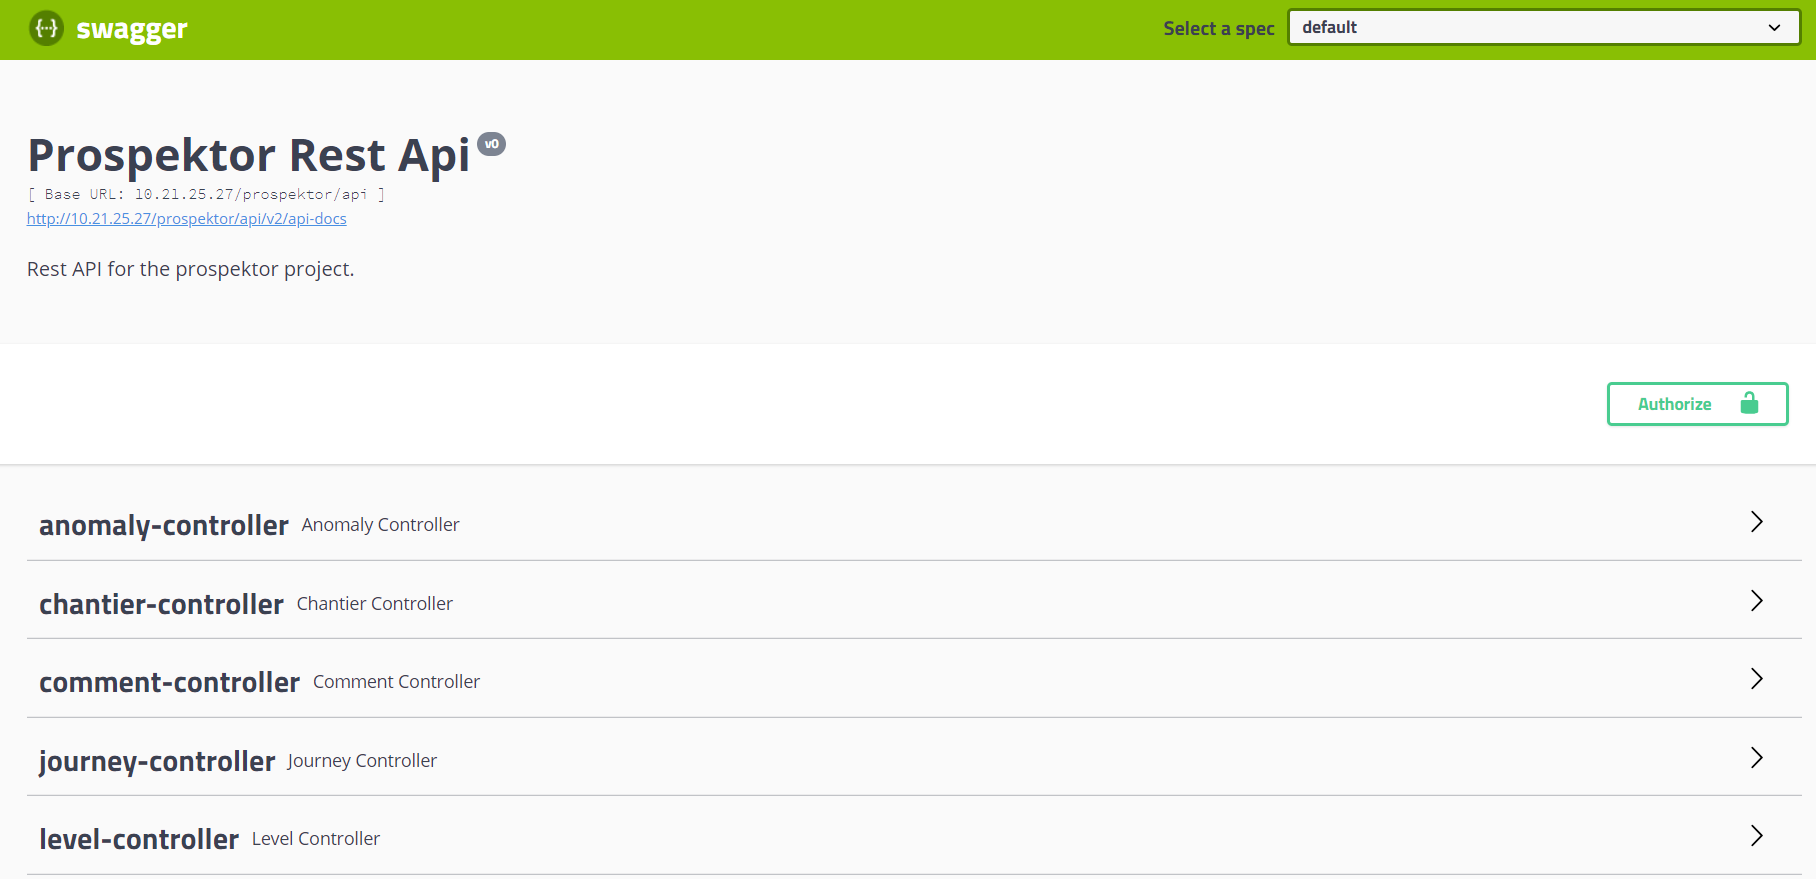
\includegraphics[width=\textwidth]{Figures/swagger.PNG}}
	\caption{\label{fig:my-label} Documentation de API Prospektor}
\end{figure}

\item \gls{JWT} : est une normalisation permettant d'utiliser des jetons pour s'authentifier sur le Web en g\'en\'eral. Il est robuste et peut contenir beaucoup d'informations. Comme tout autre jeton, JWT peut \^etre utilis\'e pour transmettre l'identit\'e d'utilisateurs authentifi\'es entre un fournisseur d'identit\'e et un fournisseur de services. Il peut \'egalement contenir toutes les revendications de l'utilisateur, telles que les donn\'ees d'autorisation. Le fournisseur de services n'a donc pas besoin d'entrer dans la base de donn\'ees ou dans des syst\`emes externes pour v\'erifier les r\^oles et autorisations des utilisateurs pour chaque demande. Ces donn\'ees sont extraites du jeton.

\end{itemize}

Choisir JWT pour s\'ecuriser nos points de terminaison d'API est un excellent choix car il garantit un \'echange sans \'etat de jetons entre le client et le serveur, est compact et s\'ecuris\'e pour les URL. Avec JWT, il est inutile de stocker les jetons d'acc\`es dans une base de donn\'ees (bien que vous puissiez toujours le faire et m\^eme en avoir besoin en fonction du cas d'utilisation) ou de nous soucier des sessions bloqu\'ees, cela rend la construction de redondance dans notre application d'entreprise plus rentable au moins aussi rentable. 

\begin{figure}[H]
	\center{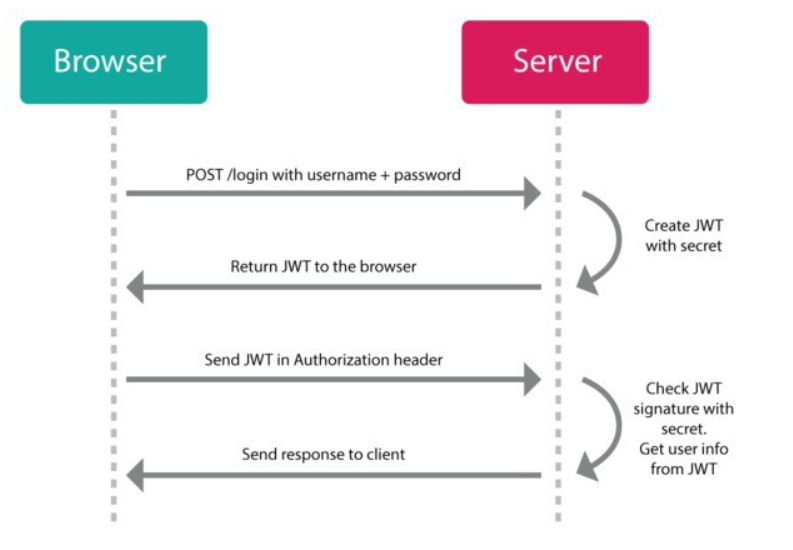
\includegraphics[width=\textwidth]{Figures/apiback.PNG}}
	\caption{\label{fig:my-label} Authentification avec JWT}
\end{figure}

On a pris Postman comme outil pour test notre \gls{API} et v\'erifier le bon fonctionnement du partie backend.

\begin{figure}[H]
	\center{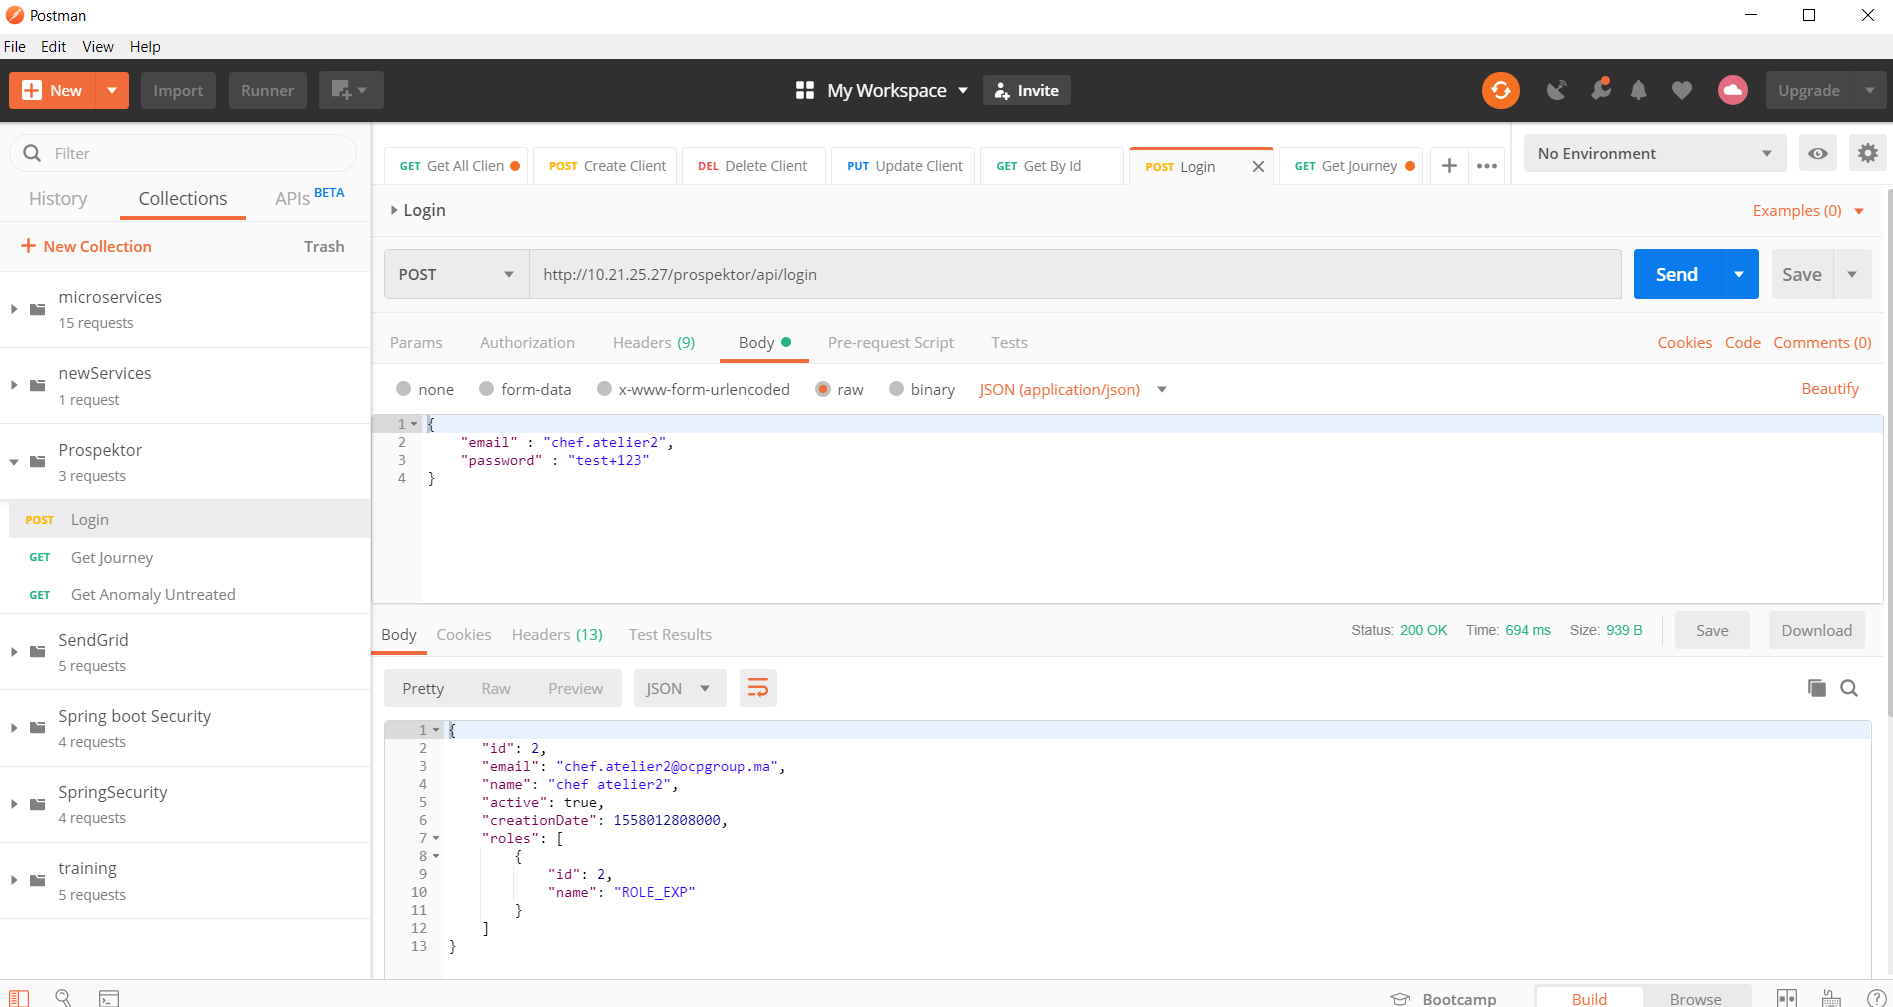
\includegraphics[width=\textwidth]{Figures/postman.PNG}}
	\caption{\label{fig:my-label} Prospektor avec Postman}
\end{figure}

\subsection{Couche FrontEnd}

On a suivre \textbf{Material Design} dans toutes les interfaces de notre application (est un ensemble de r\`egles de design propos\'ees par \textbf{Google} et qui s'appliquent \`a l'interface graphique des logiciels et applications).

Cette couche d\'ecompose \`a deux parties :

\subsubsection{Couche FrontOffice}

Pour la partie frontOffice, on a une application mobile d\'evelopp\'e par android native, utilisant le langage JAVA pour une tablette sp\'ecifique utiliser dans les chantiers du groupe \gls{OCP}. 

pourquoi android native ? 

\begin{itemize}
\item Meilleure rapidit\'e, fiabilit\'e et dot\'ee d'une meilleure r\'eactivit\'e ainsi qu'une r\'esolution sup\'erieure ce qui assure une meilleure exp\'erience utilisateur.
\item Elle permet un acc\`es plus facile \`a toutes les fonctionnalit\'es du t\'el\'ephone, de l'acc\'el\'erom\`etre en passant par la cam\'era et m\^eme le micro.
\item Les notifications push, uniquement disponibles sur les apps native. Ces notifications nous permettent d'alerter nos utilisateurs et d'attirer leur attention chaque fois que nous le souhaitons, que ce soit pour du nouveau contenu ou une offre promotionnelle.
\item Ne requiert pas forc\'ement internet pour fonctionner, ce qui est un r\'eel avantage. Dans notre cas, il existe des zones tr\`es peu couvertes par le r\'eseau internet, et permettre \`a nos utilisateurs d'acc\'eder \`a l'app sans connexion web est un tr\`es gros point fort \`a ne pas n\'egliger.
\end{itemize}

\subsubsection{Couche BackOffice}
\begin{itemize}

\item \textcolor{react}{ReactJS} : est essentiellement une biblioth\`eque JavaScript open-source qui est utilis\'ee pour cr\'eer des interfaces utilisateur sp\'ecifiquement pour les applications \`a page unique. React nous permet \'egalement de cr\'eer des composants d'interface utilisateur r\'eutilisables.

\item \textcolor{redux}{Redux} : Biblioth\`eque compl\'ementaire \`a React qui permet de conserver facilement les donn\'ees (State) et les \'ev\'enements (Actions) .Redux isole l'objet d'\'etat des composants.

\item \textbf{Redux-saga} : est une biblioth\`eque de middleware redux con\c{c}ue pour simplifier la gestion des effets secondaires de votre application redux. Pour ce faire, il exploite une fonctionnalit\'e de l'ES6 appel\'ee Generators, qui nous permet d'\'ecrire un code asynchrone qui a l'air synchrone et qui est tr\`es facile \`a tester.
\end{itemize}


Pourquoi int\'egrer ReactJS dans Prospektor ?

\begin{enumerate}
\item Le contenu est r\'ef\'eren\c{c}able

Gr\^ace \`a l'utilisation d'un serveur Node, le code va pouvoir \^etre g\'en\'er\'e c\^ot\'e client ET c\^ot\'e serveur \`a la diff\'erence des autres frameworks JS traditionnels (Backbone.js, AngularJS, Ember.js, etc.) qui de mani\`ere native ex\'ecutent le code seulement c\^ot\'e client. Jusqu'\`a pr\'esent il \'etait obligatoire de faire passer un bot (service gratuit ou payant) pour qu'il cr\'ee des fichiers HTML r\'ef\'eren\c{c}ables.

\item ReactJS est tr\`es rapide

ReactJS cr\'ee son propre DOM virtuel o\`u sont rattach\'es vos composants. Cette approche nous donne \'enorm\'ement de flexibilit\'e et des performances exceptionnelles, car ReactJS calcule quel changement dans le DOM a besoin d'\^etre fait, et change juste LA PARTIE qui a besoin d'\^etre mise \`a jour. De cette fa\c{c}on, ReactJS \'evite des op\'erations co\^uteuses dans le DOM.

\item Les composants sont le futur du d\'eveloppement web

ReactJS \`a pris le concept de Shadow DOM et du framework PolymerJS et l'a pouss\'e \`a un niveau sup\'erieur. React.js n'utilise pas Shadow DOM \`a la place il nous donne l'habilit\'e de cr\'eer nos propre composant que nous pourrons r\'eutiliser plus tard, combiner, et/ou inclure dans le c\oe{}ur de notre contenu. Cette fonctionnalit\'e \`a elle seule est un gage de productivit\'e de par la facilit\'e \`a d\'efinir et manipuler nos propres composants.

\item L'intelligibilit\'e

ReactJS produit du code ( propre ) (simple \`a lire), sa lecture permet de d\'eterminer imm\'ediatement quelles sont les fonctionnalit\'es de notre application. Ce qui est essentiel pour la maintenance et l'expansion de notre projet dans le temps.

\item Le Javascript plus simple \`a \'ecrire

ReactJS utilise une syntaxe sp\'eciale appel\'e JSX, qui permet de mixer l'HTML et le Javascript. Ce n'est pas obligatoire, nous pouvons toujours \'ecrire notre app ReactJS en Javascript natif, mais nous sugg\'erons tr\`es fortement d'essayer cette nouvelle syntaxe car elle nous permet d'\'ecrire nos composants tr\`es facilement. \^etre capable de mettre une touche de HTML dans nos fonctions de rendu sans avoir \`a concat\'ener nos chaines, c'est fantastique ! Et apr\`es quelque temps cela devient tr\`es naturel.

\end{enumerate}


\subsection{Couche Base de donn\'ees}
\begin{itemize}
\item \textbf{MySQL} : est un syst\`eme de gestion de base de donn\'ees relationnelle open source bas\'e sur le langage \gls{SQL}. Leur utilit\'e est faire stocker les donn\'ees textuel de notre application.
\item \textbf{MINIO} : est un serveur de stockage d'objets haute performance compatible avec les API Amazon S3. Pour faire stocker les attachements de l'application ( images \& audios ).
\end{itemize}

\subsection{Outils de DevOps}

\begin{itemize}
\item \textbf{Docker} : est un outil con\c{c}u pour faciliter la cr\'eation, le d\'eploiement et l'ex\'ecution d'applications \`a l'aide de conteneurs. Les conteneurs permettent \`a un d\'eveloppeur de conditionner une application avec toutes les pi\`eces dont il a besoin, telles que des biblioth\`eques et autres d\'ependances, et de l'exp\'edier dans un package unique.

\item \textbf{Kubernetes} : est un syst\`eme d'orchestration de conteneur open-source permettant d'automatiser le d\'eploiement, la mise \`a l'\'echelle et la gestion des applications.

\end{itemize}

\section{Impl\'ementation \& tests}

Nous avons r\'eparti le travail en plusieurs it\'erations (Sprints). Le sprint est un bloc de temps (1 semaine) durant lequel un incr\'ement du produit sera r\'ealis\'e. Tous les sprints ont le m\^eme dur\'ee et ne chevauchent jamais. Tout au long de cette partie, on va traiter le sprint 5 "Cr\'eer un chantier" comme mod\`ele pour tous les autres sprints, puis on va donner des captures d'\'ecran de la r\'esultat courant du notre projet avec les tests de validation.

\subsection{Sprint mod\`ele : Cr\'eer un chantier}

\subsubsection{Description g\'en\'erale du sprint}

Au cours de ce sprint nous sommes focalis\'es sur la cr\'eation d'un chantier. Dans un premier temps, on va afficher une \'ecran qui permet au utilisateur de remplir les \'el\'ements n\'ecessaire pour cr\'eer un chantier. Cette sprint se base sur la partie frontOffice (concernant l'utilisateur de l'application mobile).

\subsubsection{Description d\'etaille du sprint}

Apr\`es l'authentification, le prospecteur passe \`a l'\'ecran d'accueil. Puis, il peut suivre les d\'emarches suivantes :
\begin{figure}[H]
	\center{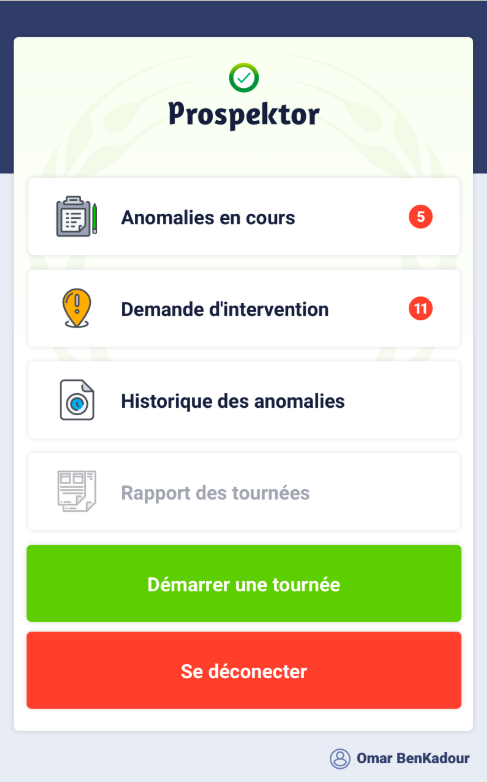
\includegraphics[width=0.4\textwidth]{Figures/acceuil.PNG}}
	\caption{\label{fig:my-label} Ecran d'acceuil}
\end{figure}
\begin{itemize}
\item Prospecteur peut cliquer sur le button (D\'emarrer une tourn\'ee).
\item la tablette envoie au serveur une requ\^ete pour g\'en\'erer un chantier vide et recevoir leur identifiant.
\item Passant \`a l'autre \'ecran qui contient les d\'etails d'un chantier.
\item Avant l'affichage de l'\'ecran, la tablette demande au serveur toutes les informations sur les machines, zones, trench\'ees \& sorties d'une mine sp\'ecifique.
\item Apr\'es la r\'eception de ces informations, l'\'ecran sera afficher et le prospecteur peut remplir les champs de chantier d'une fa\c{c}on ordonn\'ee.
\begin{figure}[H]
	\center{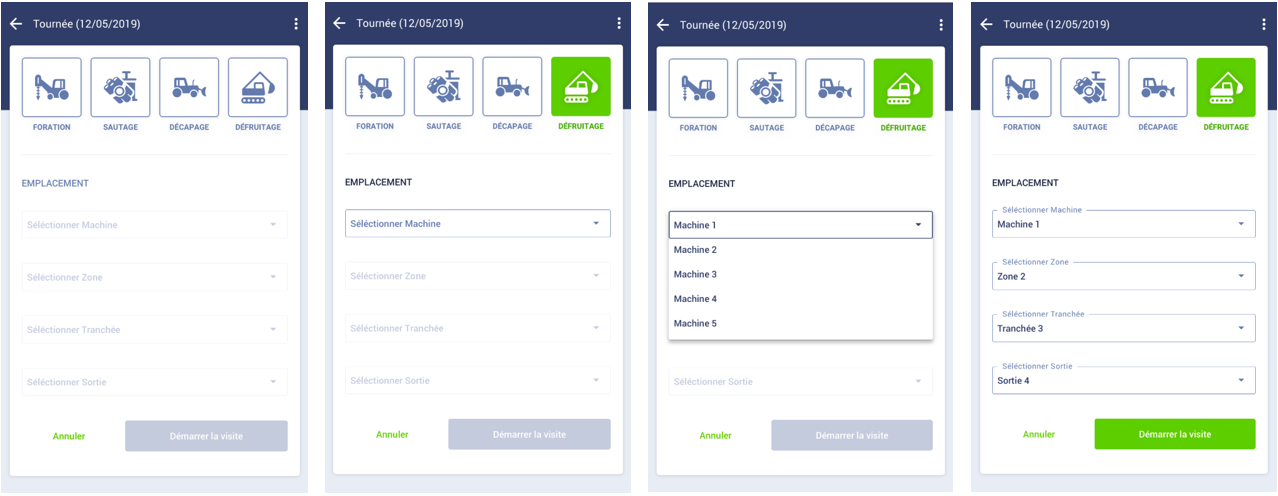
\includegraphics[width=\textwidth]{Figures/chantier.PNG}}
	\caption{\label{fig:my-label} \'Ecran de chantier}
\end{figure}
\item Enfin, une button pour la  confirmation.
\item une requ\^ete sera envoy\'e au serveur qui contient tout les informations sur ce chantier.
\end{itemize} 

On a d\'eveloppe les derni\`eres \'ecran par android studio. respectant l'architecture \gls{MVP} qu'on a d\'ej\`a expliqu\'e.

\begin{figure}[H]
	\center{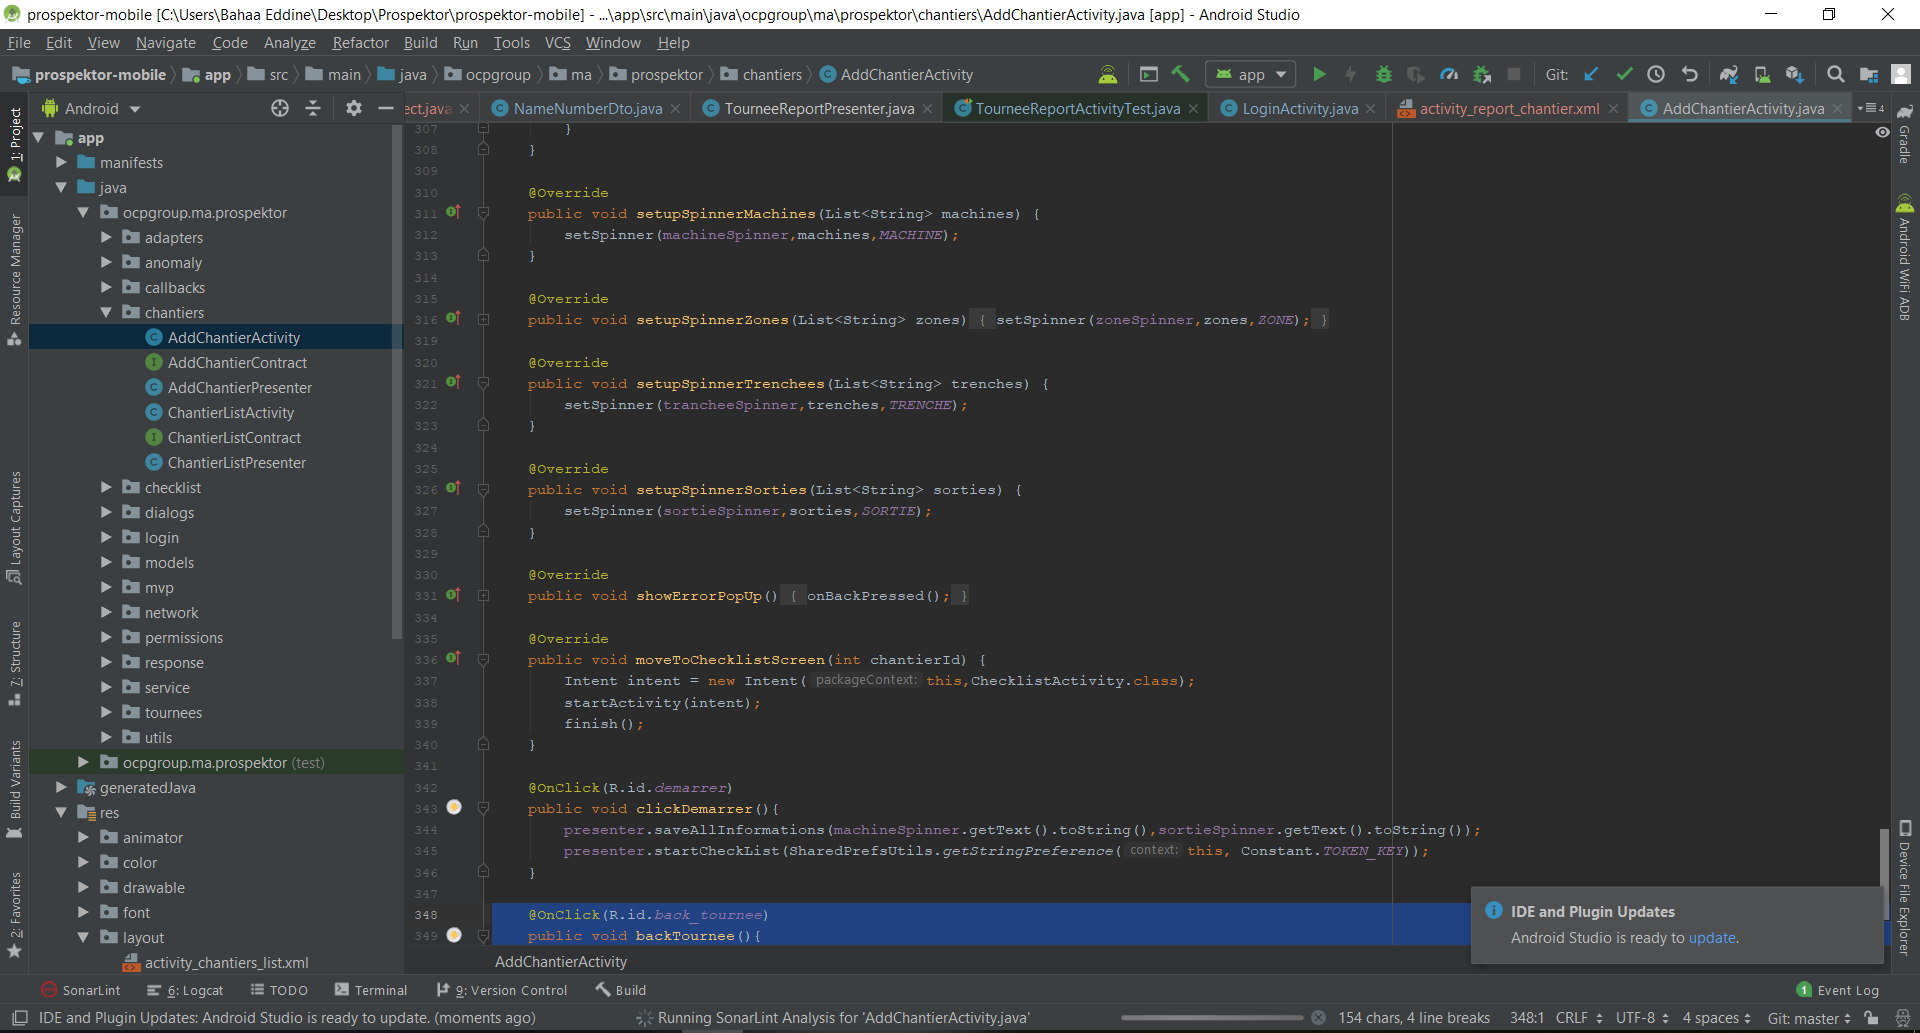
\includegraphics[width=\textwidth]{Figures/androidstudio.PNG}}
	\caption{\label{fig:my-label} Outil Android Studio}
\end{figure}

\subsection{Captures d'\'ecran du r\'esultat courant}

Pour la r\'esultat courant de notre application. On va concentrer sur la partie frontoffice, c'est la partie importante dans notre projet qui suive les proc\'edures suivantes : 

\subsubsection{Prospecteur WorkFlow}

Lors d'authentificattion comme prospecteur, l'utilisateur peut suivre les \'ecrans suivantes :

\begin{figure}[H]
	\center{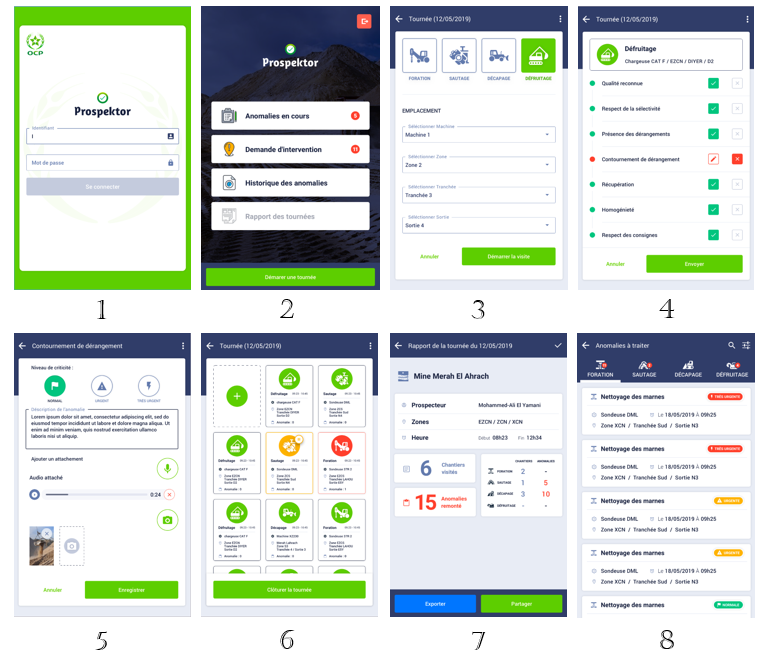
\includegraphics[width=\textwidth]{Figures/workflowprospector.PNG}}
	\caption{\label{fig:my-label} Prospecteur WorkFlow}
\end{figure}

\begin{enumerate}
\item \textbf{Authentification} : Insertion du nom d'utilisateur \& mot de passe.

\item \textbf{Page d'accueil} : Pouvoir de choisir l'un des options propos\'es ou de d\'emarrer une nouvelle tourn\'ee. 

\item \textbf{Cr\'eation d'un chantier} : Remplissage les d\'etails d'un nouveau chantier.

\item \textbf{Checklist d'un chantier} : V\'erification des r\'egl\'es d'un chantier par phase lors d'extraction des phosphates.

\item \textbf{Cr\'eation d'une anomalie \& Ajouter des attachements} : Cr\'eer une anomalie par leur criticit\'e \& ajouter des attachements (photo ,audio) pour plus clarifier le probl\`eme.

\item \textbf{liste des chantiers} : L'affichage d\'etailles de tous les chantiers par la tourn\'ee courante.

\item \textbf{Rapport d'une tour\'ee} : Avoir le rapport de la tourn\'ee apr\`es leur cl\^oturation.

\item \textbf{liste des anomalies} : L'affichage d\'etailles de toutes les anomalies.
\end{enumerate}

\subsubsection{Exploitant WorkFlow}

Lors d'authentificattion comme exploitant, l'utilisateur peut suivre les \'ecrans suivantes :

\begin{figure}[H]
	\center{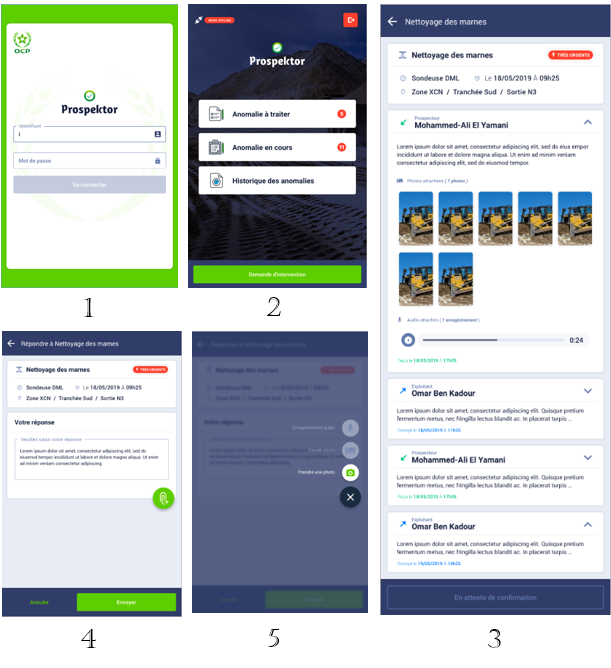
\includegraphics[width=\textwidth]{Figures/workflowexploitant.PNG}}
	\caption{\label{fig:my-label} Exploitant WorkFlow}
\end{figure}

\begin{enumerate}
\item \textbf{Authentification} : Insertion du nom d'utilisateur \& mot de passe.

\item \textbf{Page d'accueil} : Pouvoir de choisir l'un des options propos\'es.

\item \textbf{liste des anomalies cr\'eer par les prospecteurs} : L'affichage d\'etailles de toutes les anomalies ainsi par leur cr\'eateur (prospecteur).

\item \textbf{R\'epondre \`a une anomalie \& Ajouter des attachements} : Apr\`es l'examination d'une anomalie cite dans la liste, le prospecteur peut r\'epondre sur cette anomalie ainsi  ajouter des attachements (photo ,audio) pour plus clarifier leur intervention (solution ou bien clarification du probl\`eme).

\end{enumerate}

\subsection{Tests de validation}

Les tests nous permettent de v\'erifier les fonctionnalit\'es de notre syst\`eme et avoir une bonne qualit\'e de notre produit. On a utilis\'e quelques frameworks et biblioth\`eque pour tester notre application.

\begin{table}[H]
\begin{center}
\begin{tabularx}{\textwidth}{ |p{3.5cm}|X| }
\hline Biblio \& framework & Description \\ \hline \hline

\begin{center}

\includegraphics[width=2cm]{Figures/junit.jpg} 
\end{center}
& 
\begin{center}
JUnit est un framework de tests unitaires pour langage de programmation Java.
\end{center}
\\ \hline

\begin{center}

\includegraphics[width=2cm]{Figures/mockito.png} 
\end{center}
& 
\begin{center}
Mockito peut \`etre utilis\'e avec JUnit. Mockito vous permet de cr\'eer et de configurer des objets fictifs.
\end{center}
\\ \hline

\begin{center}

\includegraphics[width=1.5cm]{Figures/robolectric.png} 
\end{center}
& 
\begin{center}
Robolectric est une framework de test unitaire qui permet de tester les applications Android sur la machine virtuelle sans \'emulateur ni p\'eriph\'erique.
\end{center}
\\ \hline

\begin{center}

\includegraphics[width=1cm]{Figures/jest.png} 
\end{center}
& 
\begin{center}
Jest est une biblioth\`eque pour tester le code JavaScript. Il s'agit d'un projet open source g\'er\'e par Facebook et particuli\`erement adapt\'e aux tests de code JavaScript.
\end{center}
\\ \hline

\end{tabularx}
\caption{Biblioth\`eques \& FrameWorks de test}
\end{center}
\end{table}

Au cours de la r\'ealisation de la partie frontoffice, on a cr\'ee plus que 170 test unitaire (est une proc\'edure permettant de v\'erifier le bon fonctionnement d'une partie pr\'ecise d'un logiciel ou d'une portion d'un programme) pour valider notre programme et respecter les m\'etriques de test.

\begin{figure}[H]
	\center{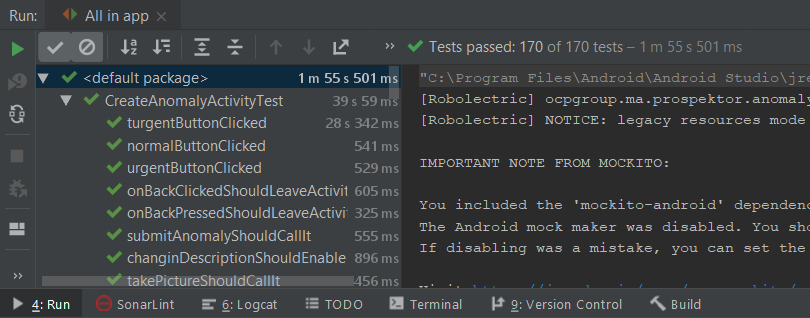
\includegraphics[width=\textwidth]{Figures/tests.PNG}}
	\caption{\label{fig:my-label} Test unitaires de la partie frontoffice}
\end{figure}

Pour v\'erifier nos tests et mesurer la qualit\'e du code source de fa\c{c}on continue de notre projet. On a utilis\'e les outils suivantes :

\begin{itemize}
\item \textbf{SonarQube} : est une plate-forme open-source d\'evelopp\'ee par SonarSource pour l'inspection continue de la qualit\'e du code afin d'effectuer des r\'evisions automatiques avec analyse statique du code afin de d\'etecter les bugs, les odeurs de code et les vuln\'erabilit\'es de s\'ecurit\'e.

\begin{figure}[H]
	\center{
\includegraphics[width=\textwidth]{Figures/sonar.PNG}}
	\caption{\label{fig:my-label} SonarQube}
\end{figure}

La \gls{DF} a d\'ej\`a configurer sonarqube pour respecter les m\'etriques suivantes :

\begin{table}[H]
\begin{center}
\begin{tabularx}{\textwidth}{ |p{5cm}|X|X|X|X| }
\hline Metric & P\'eriode de fuite & Op\'erateur & Attention & Erreur \\ \hline \hline

Bugs & No & is greater than	& & 0 \\\hline
Code Smells	& No & is greater than & 50 & 100 \\\hline
Coverage & No & is less than & 80.0\% & 30.0\% \\\hline
Duplicated Lines on New Code (\%) & Always & is greater than		& & 3.0\% \\\hline
Maintainability Rating on New Code & Always & is worse than & & A \\\hline
Reliability Rating on New Code & Always & is worse than & & A \\\hline
Security Rating on New Code & Always & is worse than & & A \\\hline

\end{tabularx}
\caption{Configuration SonarQube}
\end{center}
\end{table}


\textcolor{red}{\textbf{Remarque}} : On donne la note (Rate) suivant les r\`egles suivantes :

\begin{itemize}
\item <=5\% la note est A
\item entre 6 to 10\% la note est B
\item entre 11 to 20\% la note est C
\item entre 21 to 50\% la note est D
\item >50\% la note est E
\end{itemize}

\item \textbf{EFK Stack} : permet de cr\'eer une pile puissante pour collecter, stocker et visualiser les donn\'ees dans un emplacement centralis\'e. En effet, Fluentd, Elasticsearch et Kibana sont \'egalement connus sous le nom de EFK stack. Fluentd transf\`ere les journaux des instances individuelles du cluster vers un syst\`eme de journalisation centralis\'e, o\`u ils sont combin\'es pour g\'en\'erer des rapports de niveau sup\'erieur \`a l'aide d'ElasticSearch et de Kibana.
\end{itemize}


\begin{figure}[H]
	\center{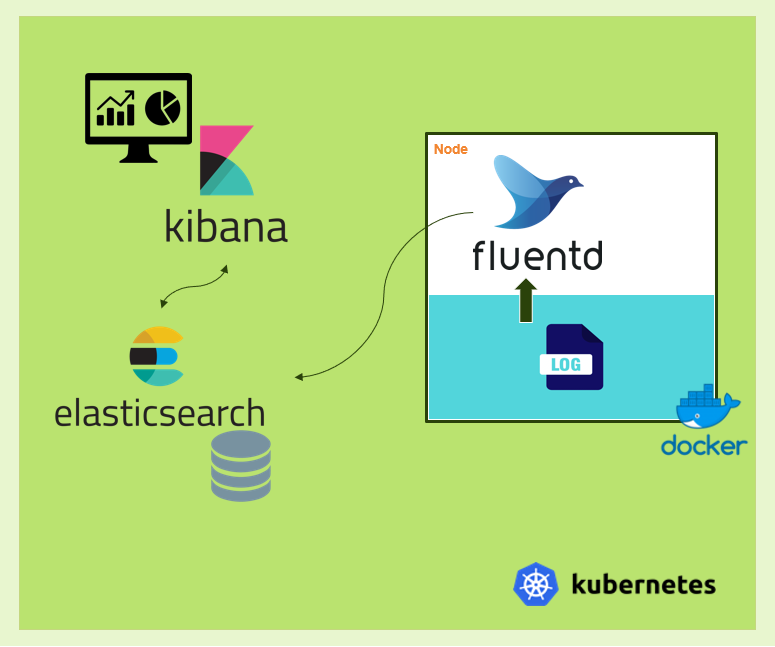
\includegraphics[width=0.6\textwidth]{Figures/efk.PNG}}
	\caption{\label{fig:my-label} EFK Stack}
\end{figure}


\subsection{D\'eploiement de projet}

L'entite \gls{DF} utilise GitLab pour offrir un emplacement pour le stockage de code en ligne et le d\'eveloppement collaboratif de projets logiciels volumineux.

\begin{figure}[H]
	\center{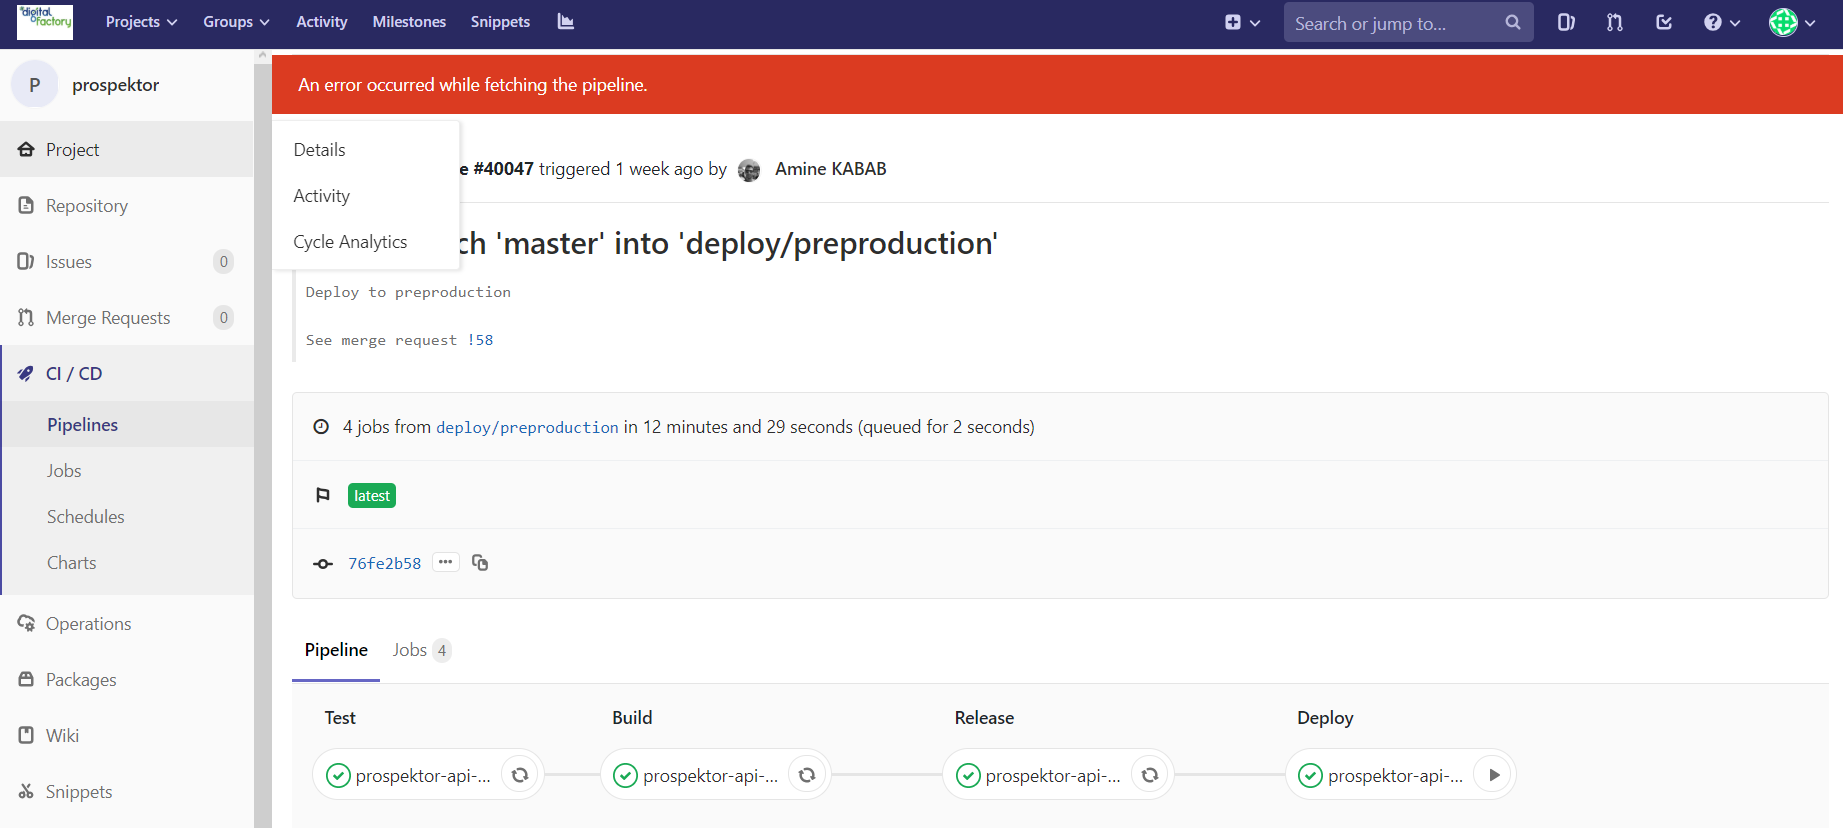
\includegraphics[width=\textwidth]{Figures/gitlab.PNG}}
	\caption{\label{fig:my-label} GitLab}
\end{figure}

Le processus de d\'eploiement que nous avons mis en place est le suivant :

\begin{figure}[H]
	\center{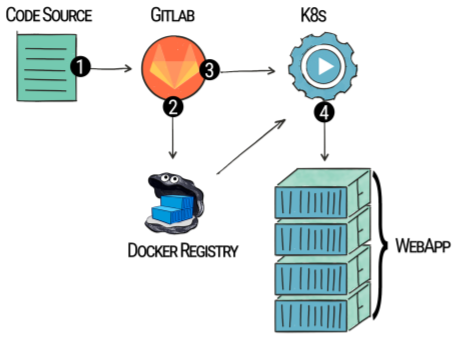
\includegraphics[width=0.7\textwidth]{Figures/deploiement.PNG}}
	\caption{\label{fig:my-label} Processus de d\'eploiement}
\end{figure}

\begin{enumerate}
\item d\'ep\^ot du code source apr\`es la validation des tests \& le lancement normale de l'application dans gitlab. 
\item cr\'eation automatique d'une image Docker et stockage dans un registre,
\item cr\'eation ou modification d'un d\'eploiement d'application dans Kubernetes,
\item d\'eploiement de l'application par Kubernetes qui cr\'ee les containers.
\end{enumerate}

\begin{figure}[H]
	\center{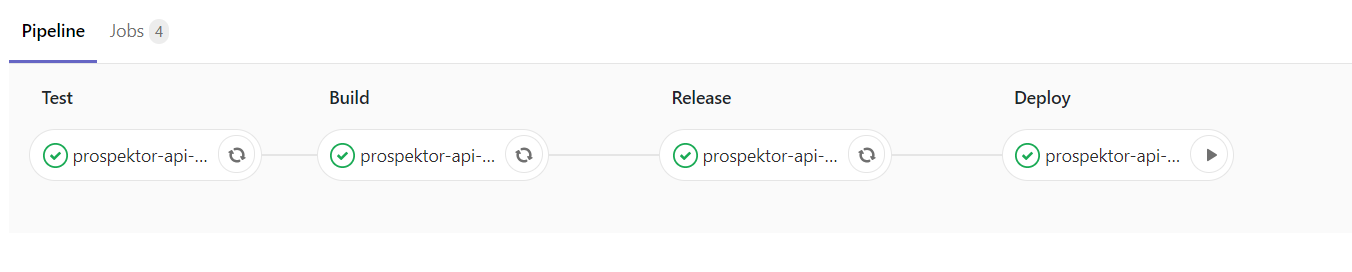
\includegraphics[width=\textwidth]{Figures/pipeline.PNG}}
	\caption{\label{fig:my-label} Pipeline de Prospektor}
\end{figure}

Ce proc\'edure est configure dans un fichier YAML ".gitlabci.yml".

\section{Conclusion}

\`A la fin de ce chapitre, nous avons r\'eussi \`a expliquer l'architecture techniques de notre system, l'\'etat d'avancement de notre projet ainsi les outils et les biblioth\`eques pour tester notre code.



